\documentclass[journal,10pt,twocolumn]{IEEEtran}

\usepackage{amsmath,amssymb,amsfonts}
\usepackage{algorithmic}
\usepackage{graphicx}
\usepackage{textcomp}
\usepackage{xcolor}
\usepackage{booktabs}
\usepackage{cite}
\usepackage{url}
\usepackage{microtype}
\usepackage{array}
\usepackage{multirow}
\usepackage{tabularx}
\usepackage{balance}
\usepackage[caption=false,font=footnotesize]{subfig}

\graphicspath{{figures/}{reports/figures/}}

\begin{document}

\title{VARDHAN: A Lightweight Dual-Domain RF-Based Framework for Drone Detection and Classification}

\author{Subash~Santhanam~K.
\thanks{The author is with the Department of Computer Science and Engineering. Project repository and verified artifacts are archived in the VARDHAN research repository.}%
}

\maketitle

\begin{abstract}
Radio frequency (RF) fingerprinting provides an effective, passive, non-line-of-sight modality for counter-unmanned aerial systems (counter-UAS) and drone surveillance. While deep learning models evaluated on the public DroneRF dataset report high classification accuracy under randomized segment-level cross-validation, their ability to generalize to unseen recording sessions remains a critical open question. In this paper, we present \textbf{VARDHAN} (\textbf{V}ersatile \textbf{A}daptive \textbf{R}adio-frequency \textbf{D}etection and \textbf{H}ierarchical \textbf{A}nalysis \textbf{N}etwork), a lightweight dual-domain architecture designed for resource-constrained edge sensing. VARDHAN-v3 processes raw 2048-sample RF waveform segments by concurrently extracting multi-scale temporal dynamics via parallel depthwise dilated convolutions ($k \in \{3, 7, 15, 31\}$, dilation $d \in \{1, 2, 4, 8\}$) and a three-channel complex Fourier representation comprising log-power spectrum, normalized real Fourier coefficients, and normalized imaginary Fourier coefficients. Branch representations are enhanced with Squeeze-and-Excitation channel attention, aggregated via learnable self-attention pooling, and interactively fused using bi-directional cross-domain gating with only \textbf{119,806} trainable parameters (11.81\,M MACs). To rigorously evaluate cross-recording robustness, we evaluate baseline architectures under both a standardized 10-fold segment-level benchmark (22,700 segments) and a strict recording-level partition (454 files across 23 sessions with zero session leakage). Under standardized segment-level evaluation, our faithful reproduction of FGCS2019DNN achieves $84.52\% \pm 0.73\%$ accuracy (macro-F1: $0.7899 \pm 0.0111$), MC1DCNN achieves $65.01\% \pm 5.35\%$ (macro-F1: $0.6207 \pm 0.0533$), and VARDHAN-v3 achieves $71.57\% \pm 1.25\%$ accuracy (macro-F1: $0.6953 \pm 0.0168$, balanced accuracy: $67.67\% \pm 2.03\%$). Conversely, under strict recording-level evaluation, accuracy across evaluated baselines drops to $26.30\%\text{--}28.77\%$ in historical benchmarks ($N_{\text{samp}}=5$) and $24.79\%$ for VARDHAN-v3 ($N_{\text{samp}}=50$, macro-F1: $0.2005$). The substantial gap between segment-level and recording-level performance is consistent with strong intra-recording correlation and recording-specific domain variation, highlighting the importance of recording-level evaluation and providing a reproducible benchmark for future domain-robust counter-UAS systems.
\end{abstract}

\begin{IEEEkeywords}
Unmanned aerial vehicles (UAVs), counter-UAS, radio frequency (RF) fingerprinting, dual-domain deep learning, temporal convolutional networks, complex spectral features, DroneRF dataset, recording leakage, edge computing.
\end{IEEEkeywords}

\section{Introduction}
\IEEEPARstart{T}{he} proliferation of low-altitude civilian and commercial Unmanned Aerial Vehicles (UAVs, commonly termed drones) has accelerated across various domains, including precision agriculture, infrastructure inspection, geographic surveying, and emergency disaster relief \cite{debas2024forensic, alsad2019rf}. However, the widespread accessibility of low-cost commercial drones poses escalating security, privacy, and safety hazards. Unauthorized drone incursions have disrupted commercial airport operations, endangered critical infrastructure, facilitated contraband smuggling across borders, and created severe airspace collision risks \cite{taha2019machine, debas2024forensic, sihag2023cyber4drone}. Consequently, developing automated, reliable, and energy-efficient counter-UAS (C-UAS) detection and classification technologies is imperative for civilian and military airspace security.

Traditional drone surveillance modalities---including primary radar, electro-optical/infrared (EO/IR) cameras, and acoustic sensor arrays---exhibit fundamental physical constraints in complex operational environments \cite{debas2024forensic, taha2019machine}. Optical and infrared cameras require unobstructed line-of-sight (LoS), adequate ambient lighting, and high-resolution optics, rendering them ineffective in fog, heavy precipitation, direct solar glare, or low-light night conditions \cite{ezuma2019micro}. Acoustic sensing is hindered by severe attenuation with distance, urban ambient acoustic noise, and aerodynamic interference from wind or vehicular traffic \cite{ezuma2020detection}. Active radar systems suffer from small radar cross-sections (RCS) of micro-drones, severe multi-path ground clutter, high equipment costs, and active RF emission footprints that reveal sensor locations \cite{taha2019machine}.

In contrast, passive Radio Frequency (RF) sensing provides a resilient surveillance modality. Consumer UAVs rely on wireless bidirectional RF communication links between the unmanned aircraft and its Ground Control Station (GCS) or remote controller to transmit telemetric data, command-and-control (C2) packets, and real-time video downlinks (predominantly within the 2.4\,GHz and 5.8\,GHz industrial, scientific, and medical (ISM) bands) \cite{alsad2019rf, allahham2019dronerf}. Intercepting these passive RF emissions enables non-line-of-sight detection over long operational ranges regardless of visual obscurity, weather, or acoustic clutter, and does not require the sensing platform to intentionally transmit RF energy.

To facilitate data-driven RF classification research, Al-Sa'd et al. \cite{alsad2019rf, allahham2019dronerf} released the public \textbf{DroneRF} dataset, containing raw high-rate RF waveform recordings from three commercial UAV models (Parrot Bebop, Parrot AR Drone 2.0, DJI Phantom 3) and background RF environments across 10 flight states. Subsequent studies \cite{alsad2019rf, allahham2020deep, mo2022deep, medaiyese2021machine, alemadi2020drone, nemer2021rf, zhang2021rf} have applied Deep Neural Networks (DNN), 1D/2D Convolutional Neural Networks (CNN), and XGBoost to DroneRF, reporting impressive classification accuracies exceeding $84\%\text{--}99\%$.

However, a critical methodological limitation underlies much of the published literature: \textit{segment-level cross-validation protocols}. In segment-level evaluation, contiguous temporal recordings are partitioned into thousands of sub-segments, and segments originating from the same physical recording session are distributed across both training and test folds. Because consecutive RF segments within a single physical session may share transmitter-, receiver-, propagation-, and environment-specific characteristics, deep networks may exploit session-specific stationary signatures rather than learning features that generalize across recording conditions. When models are subjected to \textit{strict recording-level separation}---where test segments originate entirely from unseen recording sessions---classification performance degrades substantially.

To address these challenges, this project investigates the reproducibility of published RF baselines, analyzes the cross-recording generalization gap, and proposes \textbf{VARDHAN-v3} (\textbf{V}ersatile \textbf{A}daptive \textbf{R}adio-frequency \textbf{D}etection and \textbf{H}ierarchical \textbf{A}nalysis \textbf{N}etwork), a lightweight dual-domain architecture. VARDHAN-v3 combines multi-scale temporal convolutions ($k \in \{3, 7, 15, 31\}$) with a 3-channel complex Fourier representation preserving both phase components ($\text{Re}(X)$, $\text{Im}(X)$) and log-power spectrum.

\subsection{Core Contributions}
The verified scientific contributions of this investigation are:
\begin{enumerate}
    \item \textbf{Faithful Baseline Reproduction \& Benchmarking}: We faithfully reproduce the available FGCS2019DNN \cite{alsad2019rf} implementation and construct a standardized MC1DCNN \cite{allahham2020deep} baseline from its reported architectural details alongside VARDHAN-v3 on a standardized 22,700-segment DroneRF 10-fold benchmark, and benchmark additional baseline models (DSCNN \cite{medaiyese2021machine}, Compressive Sensing CNN \cite{mo2022deep}, MobileNet-style baseline) under a strict recording-level protocol.
    \item \textbf{Strict Recording-Level Protocol}: We formulate an open-source, leak-free recording-level evaluation split (454 files, 23 sessions: 308 train / 73 val / 73 test) with zero recording or file overlap.
    \item \textbf{Lightweight Dual-Domain Architecture (VARDHAN-v3)}: We design a dual-branch neural network combining multi-scale dilated temporal convolutions, 3-channel complex Fourier representations, Squeeze-and-Excitation attention, attention pooling, and bi-directional cross-domain gating with exactly \textbf{119,806} parameters and 11.81\,M theoretical MACs.
    \item \textbf{Systematic Generalization Gap Quantification}: We present a comparative study contrasting segment-level cross-validation ($71\%\text{--}85\%$ accuracy) against unseen recording evaluation ($24\%\text{--}29\%$ accuracy), demonstrating the cross-session domain shift in RF fingerprinting.
    \item \textbf{Signal Normalization Analysis}: We investigate the mathematical mechanism of global fold Z-score normalization versus per-segment normalization, identifying how high-amplitude transmitters can introduce scale disparities between classes.
\end{enumerate}

\section{Related Work}
Passive RF drone detection has emerged as a major focus within wireless security and signal processing. Table~\ref{tab:literature_summary} summarizes primary published studies on the DroneRF dataset.

\begin{table*}[t]
\centering
\caption{Summary of Representative RF-Based UAV Detection Literature on DroneRF}
\label{tab:literature_summary}
\footnotesize
\begin{tabularx}{\textwidth}{
    >{\hsize=0.80\hsize\raggedright\arraybackslash}X
    >{\hsize=0.85\hsize\raggedright\arraybackslash}X
    >{\hsize=0.90\hsize\raggedright\arraybackslash}X
    >{\hsize=1.15\hsize\raggedright\arraybackslash}X
    >{\hsize=0.65\hsize\raggedright\arraybackslash}X
    >{\hsize=1.65\hsize\raggedright\arraybackslash}X
}
\toprule
\textbf{Reference} & \textbf{Published Model} & \textbf{Input Representation} & \textbf{Preprocessing Pipeline} & \textbf{Reported Performance} & \textbf{Reproduction / Benchmark Status} \\
\midrule
Al-Sa'd et al. (2019) \cite{alsad2019rf} & 4-Layer MLP (DNN) & 2048-pt stitched power spectrum & DC removal, 2048-pt FFT, $|X[k]|^2$, max-norm, MSE loss & 2-class: 99.7\%\newline 4-class: 84.5\%\newline 10-class: 46.8\% & \textbf{Faithfully Reproduced (Code-Mode, 295.8k params)}:\newline $84.52\% \pm 0.73\%$ (4-class, 10-fold) \\
Allahham et al. (2020) \cite{allahham2020deep} & Multi-Channel 1D CNN & 8 sub-bands $\times$ 256 DFT bins & 2048 DFT bins split into 8 non-overlapping 10\,MHz sub-bands & 2-class: 100\%\newline 4-class: 94.6\%\newline 10-class: 87.4\% & \textbf{Standardized Benchmark (275.9k params)}:\newline $65.01\% \pm 5.35\%$ (4-class, 10-fold) \\
Mo et al. (2022) \cite{mo2022deep} & Multi-stage DNN/CNN with CS & Compressively sensed RF ($CR \in \{0.25, 0.5, 0.75\}$) & Bernoulli MCRD sampling matrix $y = \Phi x$, stitched power spectra & 2-class: 100\%\newline 4-class: 99.6\%\newline 10-class: 99.3\% & Implemented and evaluated under historical strict benchmark (1,059,908 params) \\
Medaiyese et al. (2021) \cite{medaiyese2021machine} & XGBoost / DSCNN & Low-frequency RF spectrum / 1D waveform & Discrete wavelet transform and energy transient extraction & 2-class: 99.9\%\newline 4-class: 90.73\%\newline 10-class: 70.09\% & Evaluated under historical strict benchmark (68,228 params) \\
Debas et al. (2024) \cite{debas2024forensic} & Comprehensive Forensics Survey & Multi-modal forensics & Review of drone forensic models (CCAFM, DRFRF, ALFA, DroneRF) & Survey synthesis & Benchmark framing \& standardized metrics \\
\bottomrule
\end{tabularx}
\end{table*}

\subsection{DroneRF Dataset and Deep Learning Baselines}
Al-Sa'd et al. \cite{alsad2019rf} introduced the DroneRF dataset and established the initial benchmark using a four-layer Multi-Layer Perceptron (DNN). The authors processed 2048-point discrete Fourier transform (DFT) segments, reporting $99.7\%$ accuracy for 2-class detection (UAV presence vs. background), $84.5\%$ for 4-class drone type identification (Background, Bebop, AR, Phantom), and $46.8\%$ for 10-class flight mode classification.

Allahham et al. \cite{allahham2020deep} extended this work by proposing a Multi-Channel 1-Dimensional Convolutional Neural Network (MC1DCNN). The authors divided the 80\,MHz intercepted spectrum into eight 10\,MHz sub-bands ($8 \times 256$ bins), feeding them into parallel convolutional filter channels. They reported $94.6\%$ 4-class accuracy and $87.4\%$ 10-class accuracy under their customized split.

Mo et al. \cite{mo2022deep} integrated Compressive Sensing (CS) with deep learning, applying Multi-Channel Random Demodulation (MCRD) via Bernoulli measurement matrices ($\Phi \in \mathbb{R}^{M \times N}$) at compression ratios $CR = M/N \in \{0.25, 0.50, 0.75\}$. They reported over $99\%$ accuracy on compressively sensed spectra using multi-stage DNN/CNN classifiers.

\subsection{Literature Results vs. Project Reproductions}
It is essential to formally distinguish between \textit{published literature results} and \textit{our standardized reproductions}. Published results in \cite{alsad2019rf, allahham2020deep, mo2022deep} evaluated performance using randomized segment splits where segments from identical recording files were intermixed. In our faithful reproduction of FGCS2019DNN under a standardized 10-fold cross-validation protocol over all 22,700 segments of DroneRF, the model achieves $84.52\% \pm 0.73\%$ accuracy, closely matching the original paper's reported $84.5\%$. However, under our historical strict recording-level benchmark, the FGCS-based baseline (565,956 parameters) achieved $28.22\%$ accuracy.

\begin{figure*}[t]
\centering
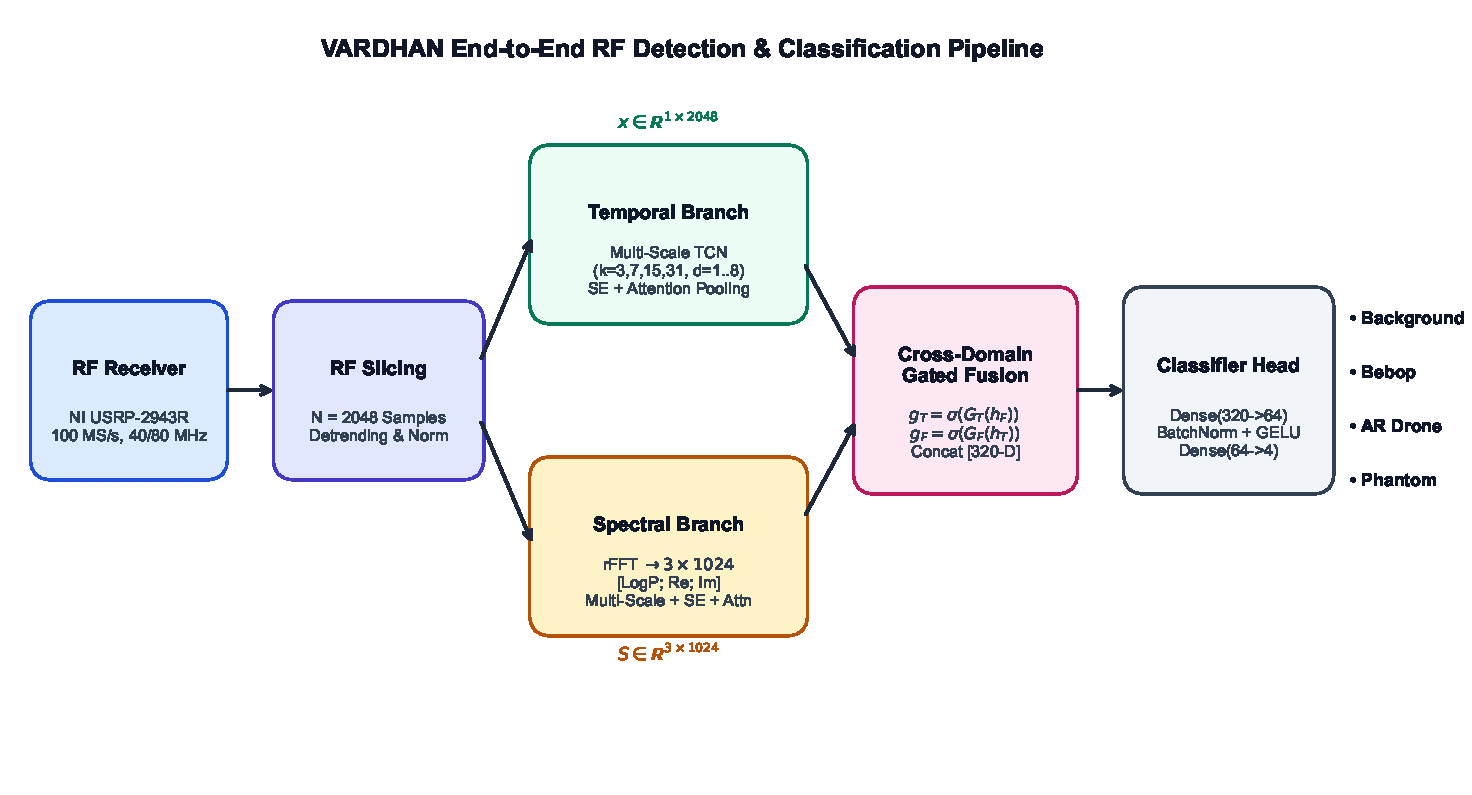
\includegraphics[width=0.98\textwidth]{figures/vardhan_overall_architecture.pdf}
\caption{End-to-end processing pipeline of the VARDHAN-v3 framework. A raw 2048-sample RF waveform slice is concurrently fed into a Multi-Scale Temporal Convolutional Network (MS-TCN) and a 3-channel complex Fourier transform branch ($S \in \mathbb{R}^{3 \times 1024}$). Features are pooled via self-attention, modulated via bi-directional cross-domain gating, and classified across four output classes.}
\label{fig:overall_arch}
\end{figure*}

\section{DroneRF Dataset and Protocol Topologies}
\subsection{Dataset Composition and Hardware Configuration}
The DroneRF dataset \cite{allahham2019dronerf} was collected using two synchronized National Instruments USRP-2943R software-defined radio (SDR) receivers. Each receiver recorded real-valued voltage amplitudes at a sampling rate of $F_s = 100\,\text{MS/s}$ with 14-bit ADC resolution across a 40\,MHz instantaneous bandwidth. Both receivers were configured to cover the 2.4\,GHz WiFi spectrum (2.40--2.48\,GHz): Receiver~1 captured the lower band ($L$, center frequency 2.422\,GHz, spanning 2.40--2.44\,GHz), while Receiver~2 recorded the upper band ($H$, center frequency 2.462\,GHz, spanning 2.44--2.48\,GHz), together covering an 80\,MHz contiguous bandwidth spanning WiFi channels 1 through 13.

The dataset consists of 454 individual CSV files representing 227 synchronized $(L, H)$ recording pairs across 23 discrete recording sessions. Each raw file contains 10,000,000 real voltage samples. The recordings represent four major RF classes:
\begin{enumerate}
    \item \textbf{Background RF Activities} (Label 0): Ambient RF noise, commercial WiFi traffic, and Bluetooth activity in the absence of UAVs (41 pairs, 82 files).
    \item \textbf{Parrot Bebop Drone} (Label 1): Bebop quadcopter operating across four flight modes: connected/on, hovering, flying without video, and flying with video streaming (84 pairs, 168 files).
    \item \textbf{Parrot AR Drone 2.0} (Label 2): AR Drone quadcopter operating across the same four flight modes (81 pairs, 162 files).
    \item \textbf{DJI Phantom 3 Standard} (Label 3): Phantom 3 quadcopter operating in connected/on mode (21 pairs, 42 files).
\end{enumerate}

Table~\ref{tab:dronerf_stats} details the dataset composition and segment distributions.

\begin{table}[t]
\centering
\caption{DroneRF Dataset Organization and Class Statistics}
\label{tab:dronerf_stats}
\scriptsize
\setlength{\tabcolsep}{2.0pt}
\begin{tabularx}{\columnwidth}{
    >{\hsize=1.30\hsize\raggedright\arraybackslash}X
    >{\hsize=0.60\hsize\centering\arraybackslash}X
    >{\hsize=0.80\hsize\centering\arraybackslash}X
    >{\hsize=0.75\hsize\centering\arraybackslash}X
    >{\hsize=1.55\hsize\centering\arraybackslash}X
}
\toprule
\textbf{Class Name} & \textbf{Label} & \textbf{CSV Files} & \textbf{Pairs} & \textbf{Segments ($N=2048$)} \\
\midrule
Background RF & 0 & 82 & 41 & 4,100 (18.06\%) \\
Parrot Bebop & 1 & 168 & 84 & 8,400 (37.00\%) \\
Parrot AR Drone & 2 & 162 & 81 & 8,100 (35.68\%) \\
DJI Phantom 3 & 3 & 42 & 21 & 2,100 (9.25\%) \\
\midrule
\textbf{Total} & -- & \textbf{454} & \textbf{227} & \textbf{22,700 (100.0\%)} \\
\bottomrule
\end{tabularx}
\end{table}

\subsection{Binary Unique Identifier (BUI) Labeling}
In DroneRF, each recording is cataloged with a 5-bit Binary Unique Identifier $\text{BUI} = [b_4 b_3 b_2 b_1 b_0]$:
\begin{equation}
\text{BUI} = [\text{msBUI}, \text{lsBUI}],
\label{eq:bui}
\end{equation}
where $\text{msBUI} \in \{000, 100, 101, 110\}$ denotes the experiment and drone type (Background, Bebop, AR, Phantom), and $\text{lsBUI} \in \{00, 01, 10, 11\}$ denotes the operational mode (on/connected, hovering, flying, video recording). Background activity is assigned $\text{BUI} = 00000$.

\subsection{Evaluation Protocol Topologies}
To evaluate model performance objectively, we define two distinct experimental protocol topologies:

\subsubsection{Standardized 10-Fold Segment-Level Protocol}
Each of the 227 synchronized recording pairs (containing 10,000,000 samples per receiver channel) is divided into 100 non-overlapping contiguous blocks of 100,000 samples each, yielding 22,700 source blocks. For the VARDHAN-v3 framework, a 2048-sample discrete-time waveform segment ($N=2048$, corresponding to $20.48\,\mu\text{s}$ at $100\,\text{MS/s}$) is extracted from each 100,000-sample block. For MC1DCNN, the corresponding discrete Fourier spectrum is channelized into eight computational sub-bands ($8 \times 256$ bins). For the faithful FGCS reproduction, the full 100,000-sample block undergoes DC mean detrending prior to 2048-point DFT computation and $Q=10$ sub-band boundary concatenation. Evaluation is performed via 10-fold Stratified K-Fold cross-validation ($\text{shuffle}=\text{True}, \text{seed}=1$), with 20,430 training examples and 2,270 testing examples per fold. Here, \textit{standardized} refers to the common dataset construction and 10-fold evaluation protocol; model-specific preprocessing and optimization settings were retained according to each implementation.

\subsubsection{Strict Recording-Level Split (Zero Leakage)}
To assess generalization to completely unseen recording sessions, the 454 files (23 discrete sessions) are partitioned into:
\begin{itemize}
    \item \textbf{Training Set}: 308 files across 15 recording sessions (Bebop: 126, AR: 120, Background: 41, Phantom: 21).
    \item \textbf{Validation Set}: 73 files across 4 recording sessions (Bebop: 21, AR: 21, Background: 21, Phantom: 10).
    \item \textbf{Testing Set}: 73 files across 4 recording sessions (Bebop: 21, AR: 21, Background: 20, Phantom: 11).
\end{itemize}
This partitioning enforces \textit{zero recording overlap} and \textit{zero file overlap} between training and evaluation splits. Notably, all 21 training files for the Phantom drone were recorded on the upper receiver $H$ (2.462\,GHz), whereas validation and test Phantom recordings were captured using lower-band $L/L1/L2$ configurations, introducing a cross-channel frequency shift domain gap.

\section{Data Processing and Mathematical Formulations}

\subsection{Generic RF Waveform Segmentation}
Let a captured discrete-time real-valued RF waveform be represented as a finite-length vector $x \in \mathbb{R}^N$ with segment length $N = 2048$ samples:
\begin{equation}
x = [x[0], x[1], \dots, x[N-1]]^T.
\label{eq:waveform}
\end{equation}

\subsection{Per-Segment Mean Detrending}
To eliminate zero-frequency DC bias and low-frequency receiver drift, sample mean detrending is applied:
\begin{equation}
\mu_x = \frac{1}{N} \sum_{n=0}^{N-1} x[n],
\label{eq:mean_detrend}
\end{equation}
\begin{equation}
x_d[n] = x[n] - \mu_x, \quad \forall n \in \{0, 1, \dots, N-1\}.
\label{eq:detrended_sig}
\end{equation}

\subsection{Per-Segment Waveform Normalization}
For amplitude-invariant representation across disparate SDR gains and propagation distances, each segment is independently standardized:
\begin{equation}
\sigma_x = \sqrt{\frac{1}{N} \sum_{n=0}^{N-1} (x_d[n])^2 + \epsilon},
\label{eq:std_seg}
\end{equation}
\begin{equation}
x_{\text{norm}}[n] = \frac{x_d[n]}{\sigma_x},
\label{eq:norm_seg}
\end{equation}
where $\epsilon = 10^{-8}$ prevents division by zero in near-silent segments.

\subsection{Complex Fourier Transform and DC Removal}
The discrete Fourier transform of the real detrended sequence $x_{\text{norm}}$ is computed via the Real Fast Fourier Transform (rFFT):
\begin{equation}
X[k] = \sum_{n=0}^{N-1} x_{\text{norm}}[n] \exp\left(-j \frac{2\pi k n}{N}\right), \quad k \in \{0, 1, \dots, N/2\}.
\label{eq:rfft}
\end{equation}
For $N=2048$, the rFFT yields 1025 complex frequency bins. The DC component at $k=0$ is discarded, leaving $K = 1024$ positive-frequency bins ($k = 1, \dots, 1024$).

\subsection{VARDHAN Three-Channel Spectral Representation}
Standard RF classifiers utilize only the magnitude-squared power spectrum $|X[k]|^2$, discarding complex phase information. In VARDHAN-v3, we construct a 3-channel spectral tensor $S \in \mathbb{R}^{3 \times 1024}$:
\begin{equation}
S = \begin{bmatrix} P[k] \\ R[k] \\ I[k] \end{bmatrix} \in \mathbb{R}^{3 \times 1024},
\label{eq:spectral_tensor}
\end{equation}
defined bin-wise for $k \in \{1, \dots, 1024\}$ by:
\begin{align}
P[k] &= \ln\left(1 + \alpha \frac{|X[k]|^2}{N}\right), \quad (\alpha = 1000), \label{eq:log_power} \\
R[k] &= \frac{\text{Re}(X[k])}{\sqrt{N}}, \label{eq:real_fft} \\
I[k] &= \frac{\text{Im}(X[k])}{\sqrt{N}}. \label{eq:imag_fft}
\end{align}
The logarithmic scaling in \eqref{eq:log_power} compresses high dynamic range transmitter spikes, while the scaled real and imaginary components in \eqref{eq:real_fft}--\eqref{eq:imag_fft} preserve frequency-domain phase information.

\begin{figure*}[t]
\centering
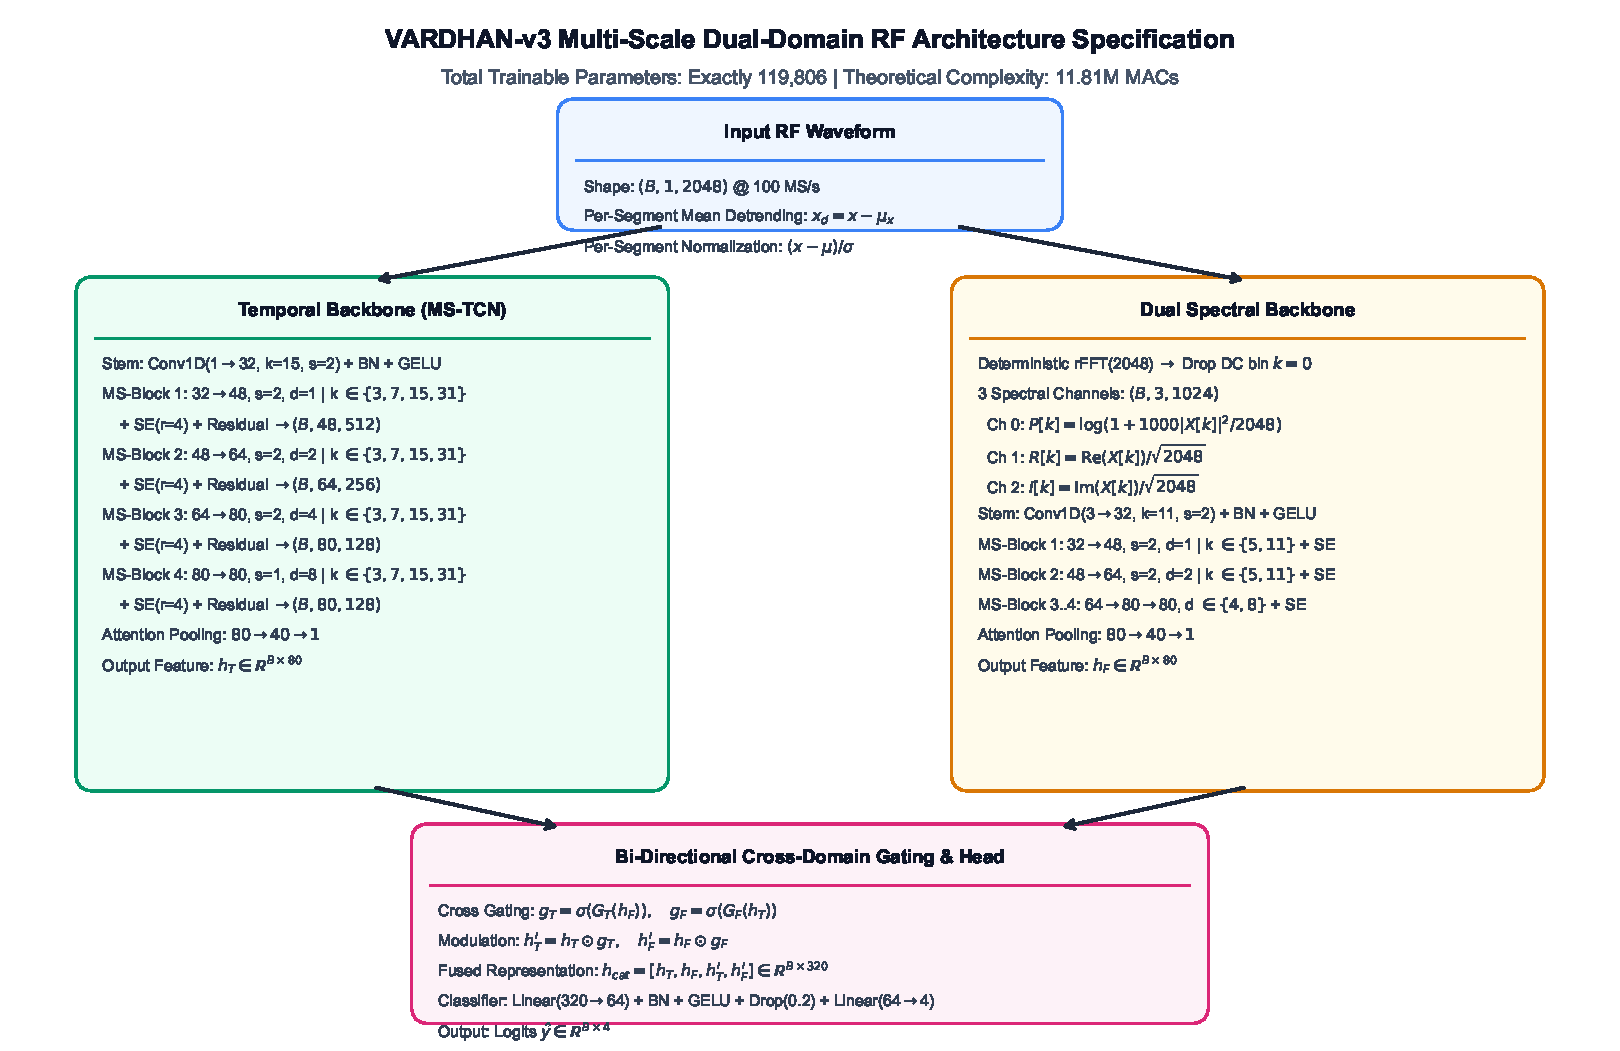
\includegraphics[width=0.98\textwidth]{figures/vardhan_detailed_architecture.pdf}
\caption{Detailed architectural blueprint of VARDHAN-v3 (119,806 trainable parameters). Left: Multi-Scale Temporal Backbone (MS-TCN) with depthwise kernel branches $k \in \{3, 7, 15, 31\}$. Right: Multi-Scale Dual Spectral Backbone with kernel branches $k \in \{5, 11\}$. Center Bottom: Bi-directional cross-domain gating and classification head.}
\label{fig:detailed_arch}
\end{figure*}

\section{Reproduction of Existing Baseline Models}
Five baseline architectures were implemented in addition to the VARDHAN models to establish comparative performance benchmarks.

\subsection{FGCS2019DNN (Al-Sa'd et al., 2019)}
\begin{itemize}
    \item \textbf{Input}: 2048-point power spectrum stitched from $L$ and $H$ bands via \cite{alsad2019rf}:
    \begin{equation}
    y_i = [y_i^{(L)}, c \cdot y_i^{(H)}], \quad c = \frac{\sum_{q=0}^{Q-1} y_i^{(L)}(M-q)}{\sum_{q=0}^{Q-1} y_i^{(H)}(q)},
    \label{eq:stitching}
    \end{equation}
    with $Q=10$ stitching boundary points.
    \item \textbf{Architecture Configurations}:
    \begin{itemize}
        \item \textit{Code-Mode Architecture} (author-released in \texttt{Classification.py}): Dense($2048 \rightarrow 128$) $\rightarrow$ ReLU $\rightarrow$ Dense($128 \rightarrow 128$) $\rightarrow$ ReLU $\rightarrow$ Dense($128 \rightarrow 128$) $\rightarrow$ ReLU $\rightarrow$ Dense($128 \rightarrow 4$) $\rightarrow$ Sigmoid (\textbf{295,812 parameters}). Used in the faithful standardized 10-fold reproduction.
        \item \textit{Paper-Mode Architecture} (described in FGCS 2019 paper text): Dense($2048 \rightarrow 256$) $\rightarrow$ ReLU $\rightarrow$ Dense($256 \rightarrow 128$) $\rightarrow$ ReLU $\rightarrow$ Dense($128 \rightarrow 64$) $\rightarrow$ ReLU $\rightarrow$ Dense($64 \rightarrow 4$) $\rightarrow$ Sigmoid (\textbf{565,956 parameters}). Evaluated under the historical strict benchmark.
    \end{itemize}
    \item \textbf{Loss Function}: Mean Squared Error (MSE) on one-hot targets:
    \begin{equation}
    \mathcal{L}_{\text{MSE}} = \frac{1}{C} \sum_{c=1}^C (y_c - \hat{y}_c)^2.
    \label{eq:mse_loss}
    \end{equation}
    \item \textbf{Optimizer}: Adam ($\text{lr} = 0.001$), batch size 10, 200 epochs.
\end{itemize}

\subsection{MC1DCNN (Allahham et al., 2020)}
\begin{itemize}
    \item \textbf{Input}: 8 sub-band channels $\times$ 256 frequency bins ($8 \times 256$).
    \item \textbf{Architecture}: Conv1D($8 \rightarrow 32, k=11, s=2, p=5$) $\rightarrow$ ReLU $\rightarrow$ MaxPool1D(2) $\rightarrow$ Conv1D($32 \rightarrow 64, k=5, s=1, p=2$) $\rightarrow$ ReLU $\rightarrow$ MaxPool1D(2) $\rightarrow$ Flatten(2048) $\rightarrow$ Dense($2048 \rightarrow 128$) $\rightarrow$ ReLU $\rightarrow$ Dense($128 \rightarrow 4$). Total parameters: \textbf{275,940}.
    \item \textbf{Loss \& Optimizer}: Cross-Entropy Loss, Adam ($\text{lr} = 0.001$), batch size 32, 100 epochs.
\end{itemize}

\subsection{DSCNN (Depthwise Separable CNN)}
\begin{itemize}
    \item \textbf{Formulation}: Depthwise convolution followed by $1 \times 1$ pointwise projection \cite{medaiyese2021machine}:
    \begin{equation}
    y_c = w_c \ast x_c, \quad y = W_{1\times 1} \ast y_{\text{dw}}.
    \label{eq:dscnn}
    \end{equation}
    \item \textbf{Parameters}: 68,228 parameters. Input: raw 1D RF waveform ($1 \times 2048$).
\end{itemize}

\subsection{Compressive Sensing CNN (Mo et al., 2022)}
\begin{itemize}
    \item \textbf{Sampling}: Random Bernoulli projection matrix $\Phi \in \mathbb{R}^{M \times N}$ at $CR = M/N = 0.5$ ($M=1024$ measurements):
    \begin{equation}
    y = \Phi x.
    \label{eq:cs_projection}
    \end{equation}
    \item \textbf{Parameters}: 1,059,908 parameters.
\end{itemize}

\subsection{MobileNet-Style Spectrogram Baseline}
\begin{itemize}
    \item \textbf{Input}: 2D Short-Time Fourier Transform (STFT) log-spectrogram tensor ($1 \times 128 \times 32$).
    \item \textbf{Parameters}: 11,588 parameters with depthwise separable 2D convolutions.
\end{itemize}

\section{Proposed VARDHAN Framework}
The VARDHAN-v3 architecture is illustrated in Fig.~\ref{fig:overall_arch} and detailed in Fig.~\ref{fig:detailed_arch}. It comprises two parallel domain-specific feature extractors, attention pooling mechanisms, and a bi-directional cross-domain gated fusion network.

\subsection{Multi-Scale Temporal Backbone (MS-TCN)}
The temporal branch accepts the detrended, normalized waveform $x_{\text{norm}} \in \mathbb{R}^{B \times 1 \times 2048}$.
\begin{enumerate}
    \item \textbf{Temporal Stem}: Conv1D($1 \rightarrow 32, k=15, s=2, p=7$) + BatchNorm1D(32) + GELU activation, downsampling to $(B, 32, 1024)$.
    \item \textbf{Multi-Scale Temporal Blocks (MSTB)}: Four cascaded residual blocks split input channels $C_{\text{in}}$ across 4 parallel depthwise convolutional branches with kernel sizes $k \in \{3, 7, 15, 31\}$ and dilation factors $d \in \{1, 2, 4, 8\}$:
    \begin{equation}
    \text{out}_{\text{dw}} = \left[ \text{DW}_3(x_1) \,\|\, \text{DW}_7(x_2) \,\|\, \text{DW}_{15}(x_3) \,\|\, \text{DW}_{31}(x_4) \right],
    \label{eq:mstb_dw}
    \end{equation}
    where $x_i \in \mathbb{R}^{B \times (C_{\text{in}}/4) \times T}$. The concatenated output is projected via a $1 \times 1$ pointwise convolution, normalized by BatchNorm, activated via GELU, refined by Squeeze-and-Excitation (SE), and summed with a residual shortcut:
    \begin{equation}
    y_{\text{MSTB}} = \text{SE}\left(\text{GELU}\left(\text{BN}\left(W_{\text{pw}} \ast \text{out}_{\text{dw}}\right)\right)\right) + \text{Res}(x).
    \label{eq:mstb_out}
    \end{equation}
    Channel progression: $32 \rightarrow 48 \rightarrow 64 \rightarrow 80 \rightarrow 80$ at sequence lengths $512 \rightarrow 256 \rightarrow 128 \rightarrow 128$.
\end{enumerate}

\subsection{Multi-Scale Dual Spectral Backbone}
The spectral branch operates on the 3-channel Fourier tensor $S \in \mathbb{R}^{B \times 3 \times 1024}$ from \eqref{eq:spectral_tensor}.
\begin{enumerate}
    \item \textbf{Spectral Stem}: Conv1D($3 \rightarrow 32, k=11, s=2, p=5$) + BatchNorm1D(32) + GELU, downsampling to $(B, 32, 512)$.
    \item \textbf{Multi-Scale Spectral Blocks (MSSB)}: Four cascaded blocks split channels across 2 parallel depthwise branches ($k \in \{5, 11\}$) with dilation schedule $d \in \{1, 2, 4, 8\}$ and SE refinement. Channel progression: $32 \rightarrow 48 \rightarrow 64 \rightarrow 80 \rightarrow 80$.
\end{enumerate}

\subsection{Squeeze-and-Excitation (SE) Channel Attention}
For an intermediate feature map $U \in \mathbb{R}^{B \times C \times L}$, SE \cite{hu2018squeeze} calculates channel descriptors via global average pooling:
\begin{equation}
z_c = \frac{1}{L} \sum_{i=1}^L U_c[i], \quad z \in \mathbb{R}^C.
\label{eq:se_pool}
\end{equation}
Channel scaling vector $s \in \mathbb{R}^C$ is computed via a bottleneck projection ($r = 4$):
\begin{equation}
s = \sigma\left(W_2 \cdot \text{ReLU}\left(W_1 z + b_1\right) + b_2\right),
\label{eq:se_gate}
\end{equation}
and features are scaled channel-wise: $\tilde{U}_c = s_c \cdot U_c$.

\subsection{Learnable Self-Attention Pooling}
Rather than using static global average pooling, sequence features $H \in \mathbb{R}^{B \times C \times L}$ are aggregated using learnable attention weights $a \in \mathbb{R}^{B \times 1 \times L}$:
\begin{equation}
a = \text{Softmax}\left(W_{\text{att2}} \cdot \tanh\left(W_{\text{att1}} H + b_1\right) + b_2\right),
\label{eq:attn_weights}
\end{equation}
producing 80-dimensional branch summary vectors:
\begin{equation}
h_T = \sum_{l=1}^L a_T[l] \cdot H_T[l] \in \mathbb{R}^{B \times 80}, \quad h_F = \sum_{l=1}^L a_F[l] \cdot H_F[l] \in \mathbb{R}^{B \times 80}.
\label{eq:attn_pool}
\end{equation}

\subsection{Bi-Directional Cross-Domain Gated Fusion}
To enable inter-domain feature modulation, the temporal feature $h_T$ is gated by spectral context $h_F$, and the spectral feature $h_F$ is gated by temporal context $h_T$:
\begin{align}
g_T &= \sigma\left(W_gT2 \cdot \text{GELU}(W_{gT1} h_F + b_{gT1}) + b_{gT2}\right) \in \mathbb{R}^{B \times 80}, \label{eq:gate_t} \\
g_F &= \sigma\left(W_gF2 \cdot \text{GELU}(W_{gF1} h_T + b_{gF1}) + b_{gF2}\right) \in \mathbb{R}^{B \times 80}. \label{eq:gate_f}
\end{align}
Modulated representations are computed via Hadamard product:
\begin{equation}
h_T' = h_T \odot g_T, \quad h_F' = h_F \odot g_F.
\label{eq:mod_feats}
\end{equation}
The original and modulated vectors are concatenated into a 320-dimensional representation:
\begin{equation}
h_{\text{cat}} = [h_T \,\|\, h_F \,\|\, h_T' \,\|\, h_F'] \in \mathbb{R}^{B \times 320}.
\label{eq:fused_cat}
\end{equation}

\subsection{Classification Head}
The classifier head maps $h_{\text{cat}}$ to class logits $\hat{y} \in \mathbb{R}^{B \times 4}$:
\begin{equation}
z_1 = \text{Dropout}_{0.2}\left(\text{GELU}\left(\text{BN}\left(W_{\text{fc1}} h_{\text{cat}} + b_{\text{fc1}}\right)\right)\right) \in \mathbb{R}^{B \times 64},
\label{eq:head_fc1}
\end{equation}
\begin{equation}
\hat{y} = W_{\text{fc2}} z_1 + b_{\text{fc2}} \in \mathbb{R}^{B \times 4}.
\label{eq:head_fc2}
\end{equation}
During training, cross-entropy with label smoothing ($\alpha_{\text{ls}} = 0.05$) is minimized:
\begin{equation}
\mathcal{L}_{\text{CE}} = - \sum_{c=1}^C \left[(1 - \alpha_{\text{ls}}) y_c + \frac{\alpha_{\text{ls}}}{C}\right] \ln\left(\frac{\exp(\hat{y}_c)}{\sum_{j=1}^C \exp(\hat{y}_j)}\right).
\label{eq:loss_ce}
\end{equation}

\subsection{Theoretical Receptive Field and Computational Complexity}
The theoretical receptive field $R_l$ and feature jump $j_l$ through layer $l$ with kernel $k_l$, stride $s_l$, and dilation $d_l$ follow the recurrence:
\begin{equation}
R_l = R_{l-1} + (k_l - 1) d_l j_{l-1}, \quad j_l = j_{l-1} s_l.
\label{eq:rf_recurrence}
\end{equation}
For the temporal branch ($R_0=1, j_0=1$), the multi-scale branches yield a theoretical receptive field spanning \textbf{355 to 5,115 samples} ($3.55\,\mu\text{s}$ to $51.15\,\mu\text{s}$), fully covering the 2048-sample segment. The spectral branch achieves a receptive field spanning \textbf{435 to 1,071 frequency bins}.

VARDHAN-v3 contains exactly \textbf{119,806 trainable parameters}. The theoretical computational cost per 2048-sample segment is:
\begin{itemize}
    \item \textbf{Multiply-Accumulate Operations (MACs)}: 11.8144\,M MACs.
    \item \textbf{Floating-Point Operations (FLOPs)}: 23.6288\,M FLOPs.
\end{itemize}

\section{Experimental Setup}
\subsection{Hardware and Execution Environment}
Experiments were conducted using Python and PyTorch deep learning environments accelerated by NVIDIA Tesla T4 GPU hardware (16\,GB VRAM).

\subsection{Model-Specific Training Configurations}
To ensure complete reproducibility, Table~\ref{tab:training_configs} lists the verified model-specific training hyperparameter configurations across all standardized benchmark runs.

\begin{table}[t]
\centering
\caption{Model-Specific Experimental Configurations for Standardized 10-Fold Benchmark}
\label{tab:training_configs}
\scriptsize
\setlength{\tabcolsep}{2.2pt}
\begin{tabularx}{\columnwidth}{
    >{\hsize=1.05\hsize\raggedright\arraybackslash}X
    >{\hsize=0.90\hsize\centering\arraybackslash}X
    >{\hsize=0.85\hsize\centering\arraybackslash}X
    >{\hsize=1.20\hsize\centering\arraybackslash}X
}
\toprule
\textbf{Parameter} & \textbf{FGCS2019DNN} & \textbf{MC1DCNN} & \textbf{VARDHAN-v3} \\
\midrule
Architecture Mode & Code (128-128-128) & 8 Sub-bands & Dual-Domain TCN/FFT \\
Trainable Params & 295,812 & 275,940 & 119,806 \\
Optimizer & Adam & Adam & AdamW \\
Initial Learning Rate & $0.001$ & $0.001$ & $0.0003$ \\
Weight Decay & $0.0$ & $0.0$ & $10^{-4}$ \\
LR Scheduler & None (constant) & None (constant) & Cosine Annealing \\
Minimum LR & N/A & N/A & $10^{-6}$ \\
Batch Size & 10 & 32 & 32 \\
Epochs per Fold & 200 & 100 & 15 \\
Loss Function & MSELoss & CrossEntropy & CE (Label Smooth 0.05) \\
Output Activation & Sigmoid & Linear (Logits) & Linear (Logits) \\
Normalization & Per-BUI Max & Per-BUI Max & Per-Segment \\
Cross-Validation & 10-Fold Stratified & 10-Fold Stratified & 10-Fold Stratified \\
Random Seed & 1 & 1 & 1 \\
\bottomrule
\end{tabularx}
\end{table}

\textit{Note on Computational Constraint}: Due to computational-resource and execution-time constraints on cloud GPU instances, the full standardized 10-fold segment-level benchmark was completed only for FGCS2019DNN, MC1DCNN, and VARDHAN-v3.

\subsection{Strict Recording-Level Benchmark Configuration}
Strict recording-level evaluation used:
\begin{itemize}
    \item \textbf{Historical Baseline Suite}: $N_{\text{samp}} = 5$ segments per file (365 test segments), 5 epochs, Cross-Entropy Loss, seed 42.
    \item \textbf{Final VARDHAN-v3 Experiment}: $N_{\text{samp}} = 50$ segments per file (3,650 test segments: 1000 Background, 1050 Bebop, 1050 AR, 550 Phantom), 100 epochs, AdamW ($\text{lr}=0.0003$, $\text{min\_lr}=10^{-6}$), Cosine Annealing, per-segment normalization, seed 42. Checkpoint selection based on minimum validation loss.
\end{itemize}

\begin{figure*}[t]
\centering
\subfloat[Standardized 10-Fold Segment-Level Benchmark.]{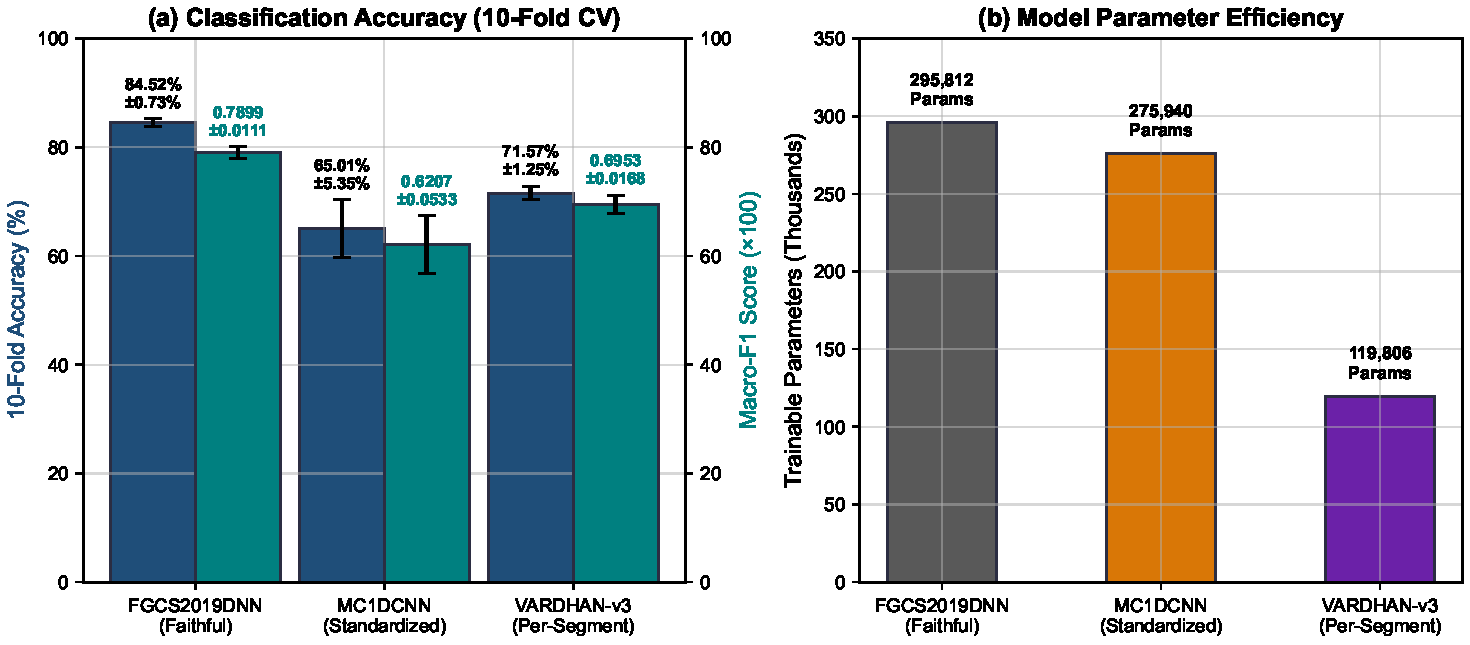
\includegraphics[width=0.48\textwidth]{figures/standardized_comparison.pdf}\label{fig:std_comp}}
\hfill
\subfloat[Historical Strict Recording-Level Benchmark.]{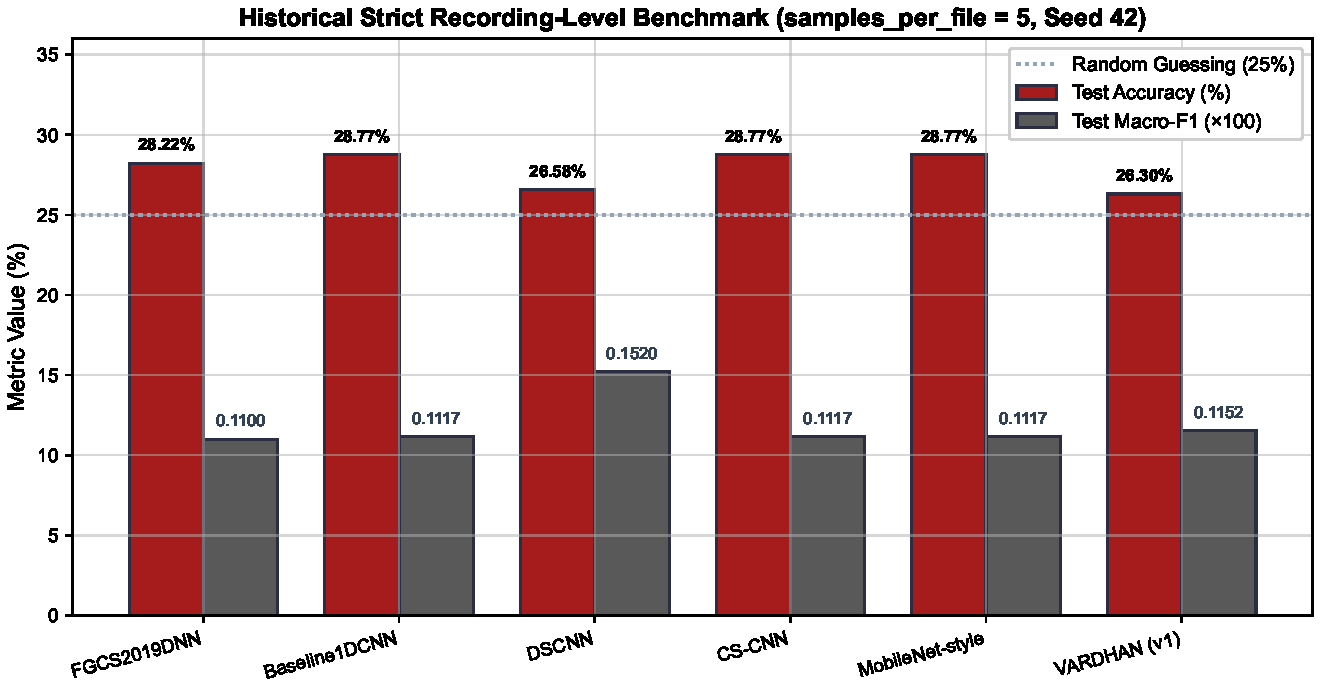
\includegraphics[width=0.48\textwidth]{figures/strict_comparison.pdf}\label{fig:strict_comp}}
\caption{Performance comparisons across evaluation protocols. (a) Standardized 10-fold segment-level benchmark ($N=22,700$). (b) Historical strict recording-level benchmark ($N_{\text{samp}}=5$, seed 42) showing severe cross-recording degradation.}
\label{fig:benchmarks}
\end{figure*}

\section{Results}

\subsection{Standardized Segment-Level Benchmark Results}
Table~\ref{tab:standardized_results} reports aggregate 10-fold cross-validation results across the 22,700 segments of DroneRF.

\begin{table}[t]
\centering
\caption{Standardized 10-Fold Segment-Level Benchmark Performance}
\label{tab:standardized_results}
\scriptsize
\setlength{\tabcolsep}{2.0pt}
\begin{tabularx}{\columnwidth}{
    >{\hsize=1.20\hsize\raggedright\arraybackslash}X
    >{\hsize=0.70\hsize\centering\arraybackslash}X
    >{\hsize=1.05\hsize\centering\arraybackslash}X
    >{\hsize=1.05\hsize\centering\arraybackslash}X
    >{\hsize=1.00\hsize\centering\arraybackslash}X
}
\toprule
\textbf{Model} & \textbf{Parameters} & \textbf{Accuracy (\%)} & \textbf{Macro-F1} & \textbf{Bal. Acc. (\%)} \\
\midrule
FGCS2019DNN \cite{alsad2019rf} & 295,812 & $\mathbf{84.52 \pm 0.73}$ & $\mathbf{0.7899 \pm 0.0111}$ & N/A \\
MC1DCNN \cite{allahham2020deep} & 275,940 & $65.01 \pm 5.35$ & $0.6207 \pm 0.0533$ & N/A \\
\textbf{VARDHAN-v3 (Ours)} & \textbf{119,806} & $71.57 \pm 1.25$ & $0.6953 \pm 0.0168$ & $\mathbf{67.67 \pm 2.03}$ \\
\bottomrule
\end{tabularx}
\end{table}

FGCS2019DNN achieves the highest segment-level accuracy ($84.52\% \pm 0.73\%$), closely matching the published literature. VARDHAN-v3 achieves $71.57\% \pm 1.25\%$ accuracy and $0.6953 \pm 0.0168$ macro-F1 while requiring \textbf{59.5\% fewer parameters} than FGCS2019DNN and \textbf{56.6\% fewer parameters} than MC1DCNN ($65.01\% \pm 5.35\%$).

\subsection{Historical Strict Recording-Level Results ($N_{\text{samp}}=5$)}
Table~\ref{tab:historical_strict} presents the historical baseline benchmark on the strict recording-level split ($N_{\text{samp}}=5$, seed 42).

\begin{table}[t]
\centering
\caption{Historical Strict Recording-Level Benchmark ($N_{\text{samp}}=5$, Seed 42)}
\label{tab:historical_strict}
\scriptsize
\setlength{\tabcolsep}{2.0pt}
\begin{tabularx}{\columnwidth}{
    >{\hsize=1.20\hsize\raggedright\arraybackslash}X
    >{\hsize=1.10\hsize\centering\arraybackslash}X
    >{\hsize=0.90\hsize\centering\arraybackslash}X
    >{\hsize=0.90\hsize\centering\arraybackslash}X
    >{\hsize=0.90\hsize\centering\arraybackslash}X
}
\toprule
\textbf{Model} & \textbf{Input Domain} & \textbf{Parameters} & \textbf{Test Acc. (\%)} & \textbf{Macro-F1} \\
\midrule
FGCS2019DNN \cite{alsad2019rf} & Power Spectrum & 565,956 & 28.22 & 0.1100 \\
Baseline1DCNN \cite{allahham2020deep} & 8 Sub-Bands & 275,940 & 28.77 & 0.1117 \\
DSCNN \cite{medaiyese2021machine} & 1D Waveform & 68,228 & 26.58 & 0.1520 \\
CS-CNN \cite{mo2022deep} & CS Measurements & 1,059,908 & 28.77 & 0.1117 \\
MobileNet-Style & 2D Spectrogram & 11,588 & 28.77 & 0.1117 \\
VARDHAN (v1) & 1D Waveform & 6,692 & 26.30 & 0.1152 \\
\bottomrule
\end{tabularx}
\end{table}

All models degrade to $26.30\%\text{--}28.77\%$ test accuracy, near the $25\%$ uniform-random four-class reference level. Macro-F1 scores ($0.1100\text{--}0.1520$) indicate that models collapse into predicting the majority class (Bebop).

\subsection{Final VARDHAN-v3 Strict Recording-Level Results ($N_{\text{samp}}=50$)}
Table~\ref{tab:v3_strict_metrics} details the final VARDHAN-v3 strict experiment ($N_{\text{samp}}=50$, 3,650 test segments, 100 epochs, per-segment normalization).

\begin{table}[t]
\centering
\caption{Final VARDHAN-v3 Strict Recording-Level Metrics ($N_{\text{samp}}=50$)}
\label{tab:v3_strict_metrics}
\scriptsize
\setlength{\tabcolsep}{2.0pt}
\begin{tabularx}{\columnwidth}{
    >{\hsize=1.35\hsize\raggedright\arraybackslash}X
    >{\hsize=0.90\hsize\centering\arraybackslash}X
    >{\hsize=0.85\hsize\centering\arraybackslash}X
    >{\hsize=0.95\hsize\centering\arraybackslash}X
    >{\hsize=0.95\hsize\centering\arraybackslash}X
}
\toprule
\textbf{Class Name} & \textbf{Precision (\%)} & \textbf{Recall (\%)} & \textbf{F1-Score (0--1)} & \textbf{Support} \\
\midrule
Background (No UAV) & 61.18 & 14.50 & 0.2344 & 1,000 \\
Parrot AR Drone & 25.28 & 19.52 & 0.2203 & 1,050 \\
Parrot Bebop Drone & 20.90 & 51.52 & 0.2974 & 1,050 \\
DJI Phantom 3 & 100.00 & 2.55 & 0.0496 & 550 \\
\midrule
\textbf{Macro Average} & \textbf{51.84} & \textbf{22.02} & \textbf{0.2005} & \textbf{3,650} \\
\midrule
\multicolumn{5}{c}{\textbf{Accuracy}: $24.79\%$ \quad \textbf{Bal. Acc.}: $22.02\%$ \quad \textbf{Loss}: $1.4735$} \\
\bottomrule
\end{tabularx}
\end{table}

\subsection{Waveform Normalization Diagnostic}
We evaluated the effect of normalization strategies on VARDHAN-v3:
\begin{itemize}
    \item \textbf{Global Train-Fold Z-Score Normalization}: Standardized 1-fold diagnostic yielded $45.55\%$ accuracy and $0.3459$ macro-F1, collapsing heavily toward Bebop (Background recall: 0.0\%, Bebop recall: 99.29\%).
    \item \textbf{Per-Segment Normalization}: Standardized 10-fold benchmark achieved $71.57\% \pm 1.25\%$ accuracy and $0.6953 \pm 0.0168$ macro-F1 (Background recall: 83.17\%, Bebop: 76.40\%, AR: 68.09\%, Phantom: 43.00\%).
\end{itemize}

\begin{figure}[t]
\centering
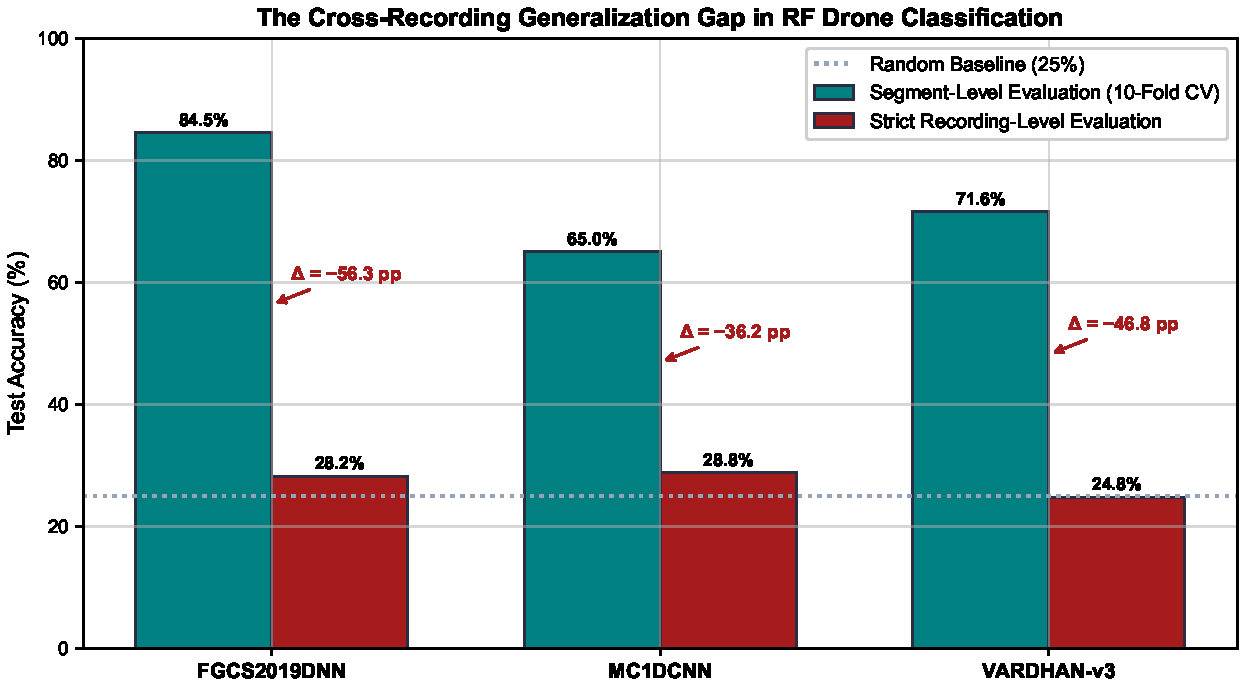
\includegraphics[width=0.48\textwidth]{figures/generalization_gap.pdf}
\caption{Cross-recording generalization gap. Segment-level evaluation produces high apparent accuracy ($65\%\text{--}85\%$), whereas strict recording-level evaluation drops to near-reference performance ($24\%\text{--}29\%$), exhibiting drops of 56.3, 36.2, and 46.8 percentage points (pp).}
\label{fig:gen_gap}
\end{figure}

\begin{figure*}[t]
\centering
\subfloat[VARDHAN-v3 Strict Training/Validation Dynamics (100 Epochs).]{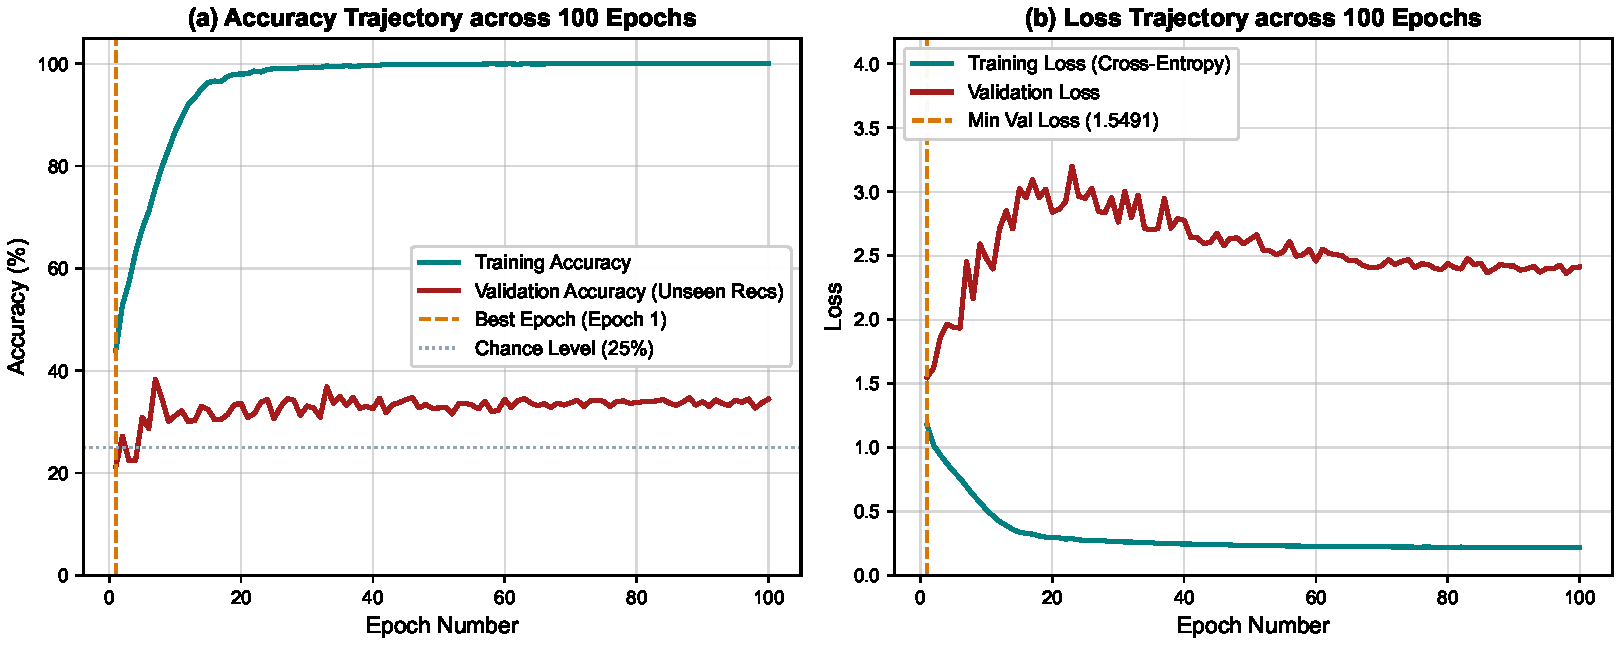
\includegraphics[width=0.48\textwidth]{figures/vardhan_training_curves.pdf}\label{fig:v3_curves}}
\hfill
\subfloat[FGCS Faithful Reproduction Confusion Matrix ($N=22,700$).]{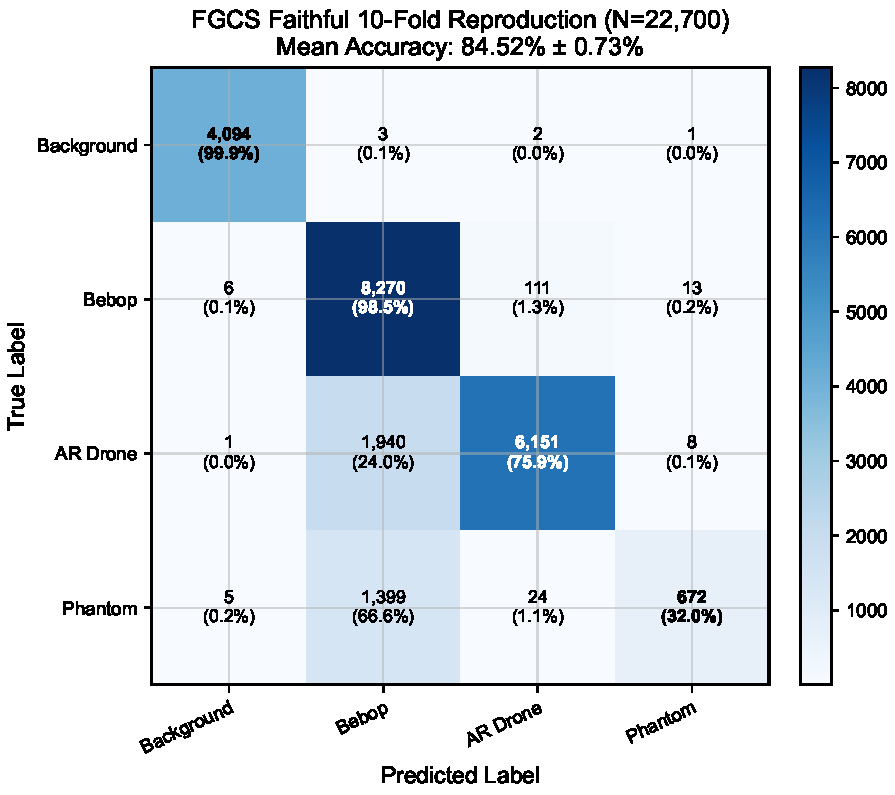
\includegraphics[width=0.48\textwidth]{figures/fgcs_confusion_matrix.pdf}\label{fig:fgcs_cm}}
\caption{Empirical error analysis. (a) Divergence between training accuracy ($100\%$) and validation accuracy ($\approx 32\%$) during strict training. (b) 10-fold confusion matrix for faithful FGCS reproduction illustrating confusion between Parrot AR / Phantom and Parrot Bebop.}
\label{fig:analysis_plots}
\end{figure*}

\section{Generalization and Error Analysis}

\subsection{The Cross-Recording Generalization Gap}
Fig.~\ref{fig:gen_gap} illustrates the cross-recording generalization gap. The performance difference between segment-level ($71.57\%$) and recording-level ($24.79\%$) represents a drop of 46.8 percentage points (pp), consistent with segment-level evaluation benefiting from strong intra-recording correlation and recording-specific domain variation. In segment-level CV, the model can exploit stationary session-level characteristics. In strict recording-level evaluation, the test sessions represent independent physical recording sessions, producing substantial out-of-distribution degradation. Possible contributors include recording-specific interference conditions, receiver characteristics, propagation effects, transmitter-specific signatures, and frequency-dependent domain shifts. These factors were not independently isolated in the present study.

\subsection{Overfitting Dynamics on Strict Protocol}
Fig.~\ref{fig:analysis_plots}(a) plots the 100-epoch training trajectory of VARDHAN-v3 on the strict split. By epoch 15, training accuracy exceeds $96\%$ ($\text{loss} < 0.33$), reaching $100.0\%$ by epoch 90. In contrast, validation accuracy remains bounded between $21\%$ and $38\%$ ($\text{loss} > 1.55$), with the minimum validation loss achieved at \textbf{Epoch 1} ($\text{val\_loss} = 1.5491$). This divergence provides clear empirical evidence of overfitting on the training sessions.

\subsection{Confusion Matrix and Normalization Scale Analysis}
Fig.~\ref{fig:analysis_plots}(b) presents the 10-fold confusion matrix for the faithful FGCS reproduction. While Background ($99.85\%$ recall, 4094/4100) and Bebop ($98.45\%$ recall, 8270/8400) are classified reliably, $23.95\%$ of AR Drone segments (1940/8100) and $66.62\%$ of Phantom segments (1399/2100) are misclassified as Bebop.

Furthermore, the diagnostic results indicate that global train-fold standardization produced substantial scale disparities between classes in this dataset, coinciding with severe Background-class degradation. Diagnostic statistics reveal that the training set standard deviation was dominated by higher-amplitude recordings ($\sigma_{\text{Phantom}} \approx 1.8835, \sigma_{\text{AR}} \approx 0.6721$), while background recordings exhibited much lower variance ($\sigma_{\text{BG}} \approx 0.0152$). Per-segment normalization addressed this scaling disparity, restoring Background recall to $83.17\%$ in VARDHAN-v3.

\section{Edge-Oriented Deployment Considerations}
VARDHAN-v3 was architected for resource-constrained edge computing. Table~\ref{tab:complexity_comparison} compares model complexity.

\begin{table}[t]
\centering
\caption{Architectural Complexity and Parameter Efficiency}
\label{tab:complexity_comparison}
\scriptsize
\setlength{\tabcolsep}{2.0pt}
\begin{tabularx}{\columnwidth}{
    >{\hsize=1.20\hsize\raggedright\arraybackslash}X
    >{\hsize=1.05\hsize\centering\arraybackslash}X
    >{\hsize=1.15\hsize\centering\arraybackslash}X
    >{\hsize=0.80\hsize\centering\arraybackslash}X
    >{\hsize=0.80\hsize\centering\arraybackslash}X
}
\toprule
\textbf{Model} & \textbf{Input Type} & \textbf{Parameters} & \textbf{MACs} & \textbf{FLOPs} \\
\midrule
CS-CNN \cite{mo2022deep} & CS ($CR=0.5$) & 1,059,908 & $\approx 54.2$\,M & $\approx 108.4$\,M \\
FGCS2019DNN \cite{alsad2019rf} & Power Spectrum & 295,812 / 565,956 & 0.30\,M & 0.59\,M \\
MC1DCNN \cite{allahham2020deep} & 8 Sub-Bands & 275,940 & 14.12\,M & 28.24\,M \\
DSCNN \cite{medaiyese2021machine} & 1D Waveform & 68,228 & 3.49\,M & 6.98\,M \\
MobileNet-Style & 2D Spectrogram & 11,588 & 1.18\,M & 2.36\,M \\
\textbf{VARDHAN-v3} & \textbf{Dual-Domain} & \textbf{119,806} & \textbf{11.81\,M} & \textbf{23.63\,M} \\
\bottomrule
\end{tabularx}
\end{table}

While VARDHAN-v3 achieves compact parameter scaling ($119.8$\,k parameters, $<0.48$\,MB FP32 model size), \textit{hardware-specific inference latency, runtime memory bandwidth, and power consumption on physical embedded hardware (e.g., NVIDIA Jetson, Raspberry Pi, ARM Cortex-M) remain unmeasured and represent future work}. Containerization and software pipelining demonstrate software deployment feasibility, but operational RF reliability requires dedicated over-the-air field validation.

\section{Limitations}
This study identifies several important limitations:
\begin{enumerate}
    \item \textbf{Dataset Scope}: DroneRF represents a controlled experimental dataset recorded with specific USRP hardware and three drone models; it does not capture diverse real-world urban RF interference.
    \item \textbf{Cross-Recording Generalization}: Performance under strict unseen recording evaluation remains low ($24.79\%$), highlighting a domain shift challenge.
    \item \textbf{Standardized Benchmark Breadth}: Full 10-fold cross-validation was completed for FGCS, MC1DCNN, and VARDHAN-v3 due to computational resource constraints.
    \item \textbf{Implementation Ambiguities}: Literature descriptions omit certain training and normalization details, necessitating faithful interpretations.
    \item \textbf{Sample Count Differences}: Historical strict baselines used $N_{\text{samp}}=5$, whereas final VARDHAN-v3 strict used $N_{\text{samp}}=50$.
    \item \textbf{Lack of External Validation}: Evaluation is confined to DroneRF without cross-dataset testing on Cardinal or private RF captures.
    \item \textbf{Hardware Latency}: Inference latency was not benchmarked on physical edge microcontrollers.
    \item \textbf{Closed-Set Constraint}: The framework assumes a closed 4-class classification space without open-set unknown drone rejection.
\end{enumerate}

\section{Future Work}
Promising future research directions include:
\begin{itemize}
    \item \textbf{Domain Adaptation \& Generalization}: Implementing adversarial domain adaptation, self-supervised pre-training (e.g., masked RF autoencoding), and cross-frequency contrastive learning to bridge recording-level domain shifts.
    \item \textbf{Data Augmentation for RF}: Applying synthetic multipath Rayleigh/Rician fading, phase noise injection, carrier frequency jitter, and SNR mixing.
    \item \textbf{Open-Set Recognition}: Designing energy-based out-of-distribution detectors and extreme value theory (EVT) classifiers to reject unknown drone models.
    \item \textbf{Hardware Optimization}: Quantizing VARDHAN-v3 to INT8/FP16 via TensorRT and ONNX Runtime for benchmarking on NVIDIA Jetson Orin and Raspberry Pi 5.
    \item \textbf{Multi-Modal Sensor Fusion}: Integrating RF fingerprinting with thermal imaging, micro-Doppler acoustic sensing, and optical camera tracking.
\end{itemize}

\section{Conclusion}
This paper presented VARDHAN, a lightweight dual-domain deep learning framework for RF-based drone detection and classification, alongside a reproducibility and generalization study on the DroneRF dataset. VARDHAN-v3 integrates multi-scale temporal convolutions ($k \in \{3, 7, 15, 31\}$) and a 3-channel complex Fourier representation with Squeeze-and-Excitation attention, attention pooling, and bi-directional cross-domain gating with exactly 119,806 parameters. Under standardized segment-level 10-fold evaluation, VARDHAN-v3 achieves $71.57\% \pm 1.25\%$ accuracy and $0.6953$ macro-F1. However, under strict unseen recording-level evaluation, accuracy across evaluated models drops to $24\%\text{--}29\%$. The observed performance gap is consistent with segment-level evaluation benefiting from intra-recording correlation and recording-specific domain variation. Furthermore, we maintain clear distinction between the historical strict baseline benchmark ($N_{\text{samp}}=5$) and the final VARDHAN-v3 strict experiment ($N_{\text{samp}}=50$). These findings emphasize the necessity of strict recording-level evaluation protocols and establish a principled foundation for future domain-robust counter-UAS research.

\bibliographystyle{IEEEtran}
\bibliography{VARDHAN_References}

\end{document}
